\section{Current Real-Data Evidence}

\paragraph{Registered 100-job study.}
The primary real-data study contains 20 locked seeds on each of BiasBios-Clinical,
Camelyon17-WILDS, CivilComments-WILDS, GaitPDB, and Waterbirds. Each job evaluates
the same 13-candidate family built with the official INLP, LEACE, R-LACE, TaCo,
and MANCE++ implementations. The strict-v2 replay reproduces all 100 decisions;
an exact-rational audit verifies 1,300 bridge certificates and 1,400 release
bounds. Table~\ref{supp:tab:current-real-rules} gives the aggregate comparison
at the primary $.40$ worst-stratum error contract.

\begin{table*}[t]
\centering
\small
\setlength{\tabcolsep}{3.7pt}
\begin{tabular}{lrrr}
\hline
Rule & Released & Estimable & Diagnostic violations \\
\hline
Strict MOSAIC & 20 & 20 & 0 \\
Direct target-table certificate & 36 & 36 & 0 \\
Bridge plug-in & 47 & 47 & 7 \\
Validation-only selection & 80 & 60 & 18 \\
Unconditional selection & 100 & 80 & 38 \\
\hline
\end{tabular}
\caption{Aggregate primary-contract outcomes over 100 registered jobs. The
direct target-table rule certifies the sampled target table; strict MOSAIC
certifies the registered bridge-admitted population class.}
\label{supp:tab:current-real-rules}
\end{table*}

Strict MOSAIC releases 20 BiasBios-Clinical interfaces at every registered
threshold from $.30$ through $.45$, and 23 interfaces at $.49$; every released
job has an estimable untouched diagnostic and no observed diagnostic violation.
The direct target-table comparator releases 36 jobs with no observed diagnostic
violation. Its guarantee applies to the target table itself, whereas MOSAIC's
bridge program certifies a structured class of target laws. The bridge plug-in,
which keeps the learned transform but omits the confidence event, releases 47
jobs and records seven diagnostic violations. This side-by-side comparison
separates target-table certification from transport certification and quantifies
the value of the simultaneous regions.

\begin{figure*}[t]
  \centering
  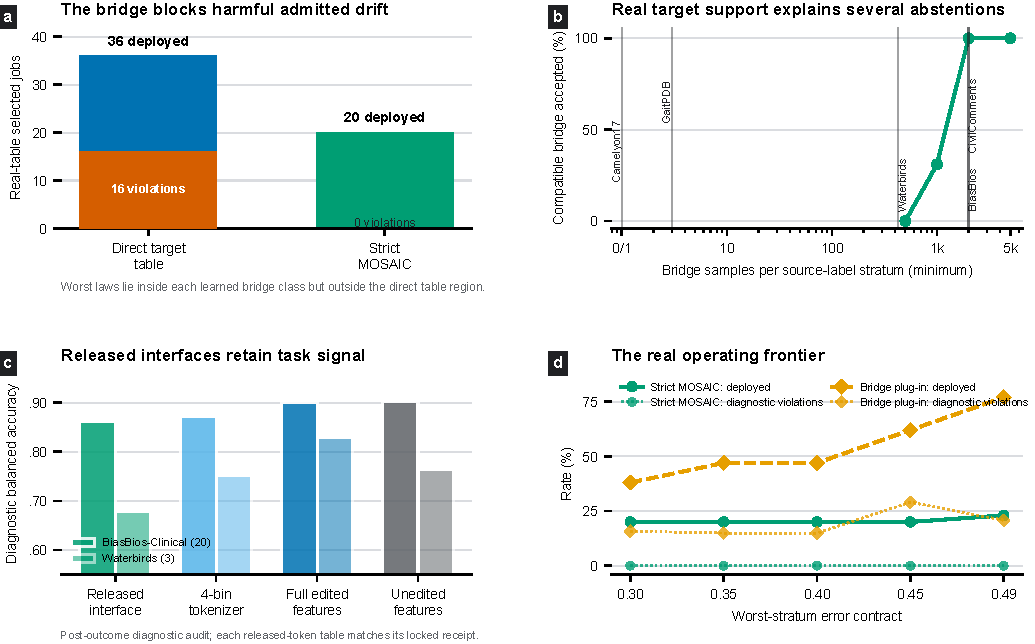
\includegraphics[width=\textwidth]{figures/figure4_mosaic_revision_evidence.pdf}
  \caption{Additional audited evidence. (a) In a post-hoc stress test under
  real-table-anchored laws in
  the learned bridge class, the direct rule violates 16/36 accepted contracts;
  MOSAIC releases 20 safely and abstains on those 16 cases. (b) Real bridge stratum support is overlaid
  on the locked bridge-power curve. (c) The released interfaces retain task
  signal on untouched diagnostics. (d) Deployment and observed
  diagnostic-violation rates across the registered utility frontier.}
  \label{supp:fig:current-real-evidence}
\end{figure*}

\paragraph{California-to-Texas confirmation.}
Five fresh ACSIncome jobs use California as the reference population and Texas
as the labeled target population. The task is income above \$50,000; binary sex
is the audit source and is excluded from released features. Five locked seeds
evaluate the complete official 13-candidate frontier. The independent strict
replay checks all 65 candidate rows and 70 global optimizations. At the $.40$
primary contract, MOSAIC abstains on all five jobs. At the registered $.45$
and $.49$ contracts, it releases all five jobs: three R-LACE and two identity
interfaces. The two identity rows are degenerate no-op releases and are not
counted as evidence that editing helped. Every released interface satisfies its
untouched Texas diagnostic. The best $.40$ errors range from $.4023$ to $.4145$.
In the active worst stratum, the bridge-residual charge is $.161$--$.211$, while
the finite-sample charge is at most $1.6\times10^{-7}$; removing the residual
charge would put every fold below $.25$. A post-review $K=8$ extension on one
previously studied seed retains only $.377$--$.540$ of the target laws. All 13
official candidates then reduce to a $.50$-error constant release and abstain.

\paragraph{Admitted-shift stress.}
The direct target-table rule and MOSAIC first see the same stored real token
tables. For each direct deployment, we then choose residual simplex vertices
that maximize that release's Bayes source attacker and form
$q^*=t\widehat pT+(1-t)r^*$. Reconstruction error is zero, so every $q^*$ lies
inside the candidate's learned bridge class. All 36 lie outside the direct
target confidence region. Table~\ref{supp:tab:admitted-shift} reports the
primary $.40$ outcome. This post-hoc deterministic stress was added after the
original
confirmation; it establishes a harmful law inside the certified class, not its
frequency in practice.

\begin{table}[t]
\centering
\small
\setlength{\tabcolsep}{3.4pt}
\begin{tabular}{lrrr}
\hline
Rule & Deploy & Violations & Abstain \\
\hline
Direct target table & 36 & 16 & 0 \\
Strict MOSAIC & 20 & 0 & 16 \\
\hline
\end{tabular}
\caption{Outcomes on the 36 direct-selected jobs after moving to an exact
member of each learned bridge class.}
\label{supp:tab:admitted-shift}
\end{table}

The direct violation rate is 44.4\% (exact 95\% interval $[27.9,61.9]$).
All 16 failures are Waterbirds releases; the 20 BiasBios releases remain safe.
The median maximum structural total-variation radius is $.279$, while the
median $\ell_1$ distance beyond the direct confidence region is $.359$. Across
the registered error thresholds $.30,.35,.40,.45,.49$, direct violations are
$18/20,4/20,16/36,20/40,$ and $23/43$; the candidate-matched strict MOSAIC rule
has zero violations at every threshold.

\paragraph{Released-interface utility.}
Table~\ref{supp:tab:released-utility} gives the values behind
Fig.~\ref{supp:fig:current-real-evidence}(c). Intervals are descriptive
two-sided 95\% $t$ intervals over released jobs. Every diagnostic token table
matches its locked receipt.

\begin{table*}[t]
\centering
\small
\setlength{\tabcolsep}{3.8pt}
\begin{tabular}{lcc}
\hline
Interface evaluated & BiasBios-Clinical ($n=20$) & Waterbirds ($n=3$) \\
\hline
Released stochastic interface & $.863\ [.857,.868]$ & $.678\ [.636,.721]$ \\
Four-bin tokenizer & $.873\ [.867,.878]$ & $.752\ [.673,.831]$ \\
Full edited features & $.901\ [.898,.904]$ & $.830\ [.811,.849]$ \\
Unedited features & $.903\ [.902,.905]$ & $.764\ [.745,.783]$ \\
\hline
\end{tabular}
\caption{Mean diagnostic balanced accuracy and 95\% interval. The released
interface is compact and task-specific; it is not a reusable embedding.}
\label{supp:tab:released-utility}
\end{table*}

\section{Finite-Alphabet Scaling}

The post-review scaling study crosses five fine alphabets and three source
counts with five sampled tables per cell, for 75 optimizations at $n=2000$ per
source--label stratum. All cells use two labels, two released tokens, source
advantage $.35$, utility error $.40$, and residual contamination $.05$.
Figure~\ref{supp:fig:scaling} reports every cell. All 75 releases certify at
the registered $.40$ contract. Tightening the error contract reveals the
expected retention frontier as the multinomial radius grows with $K$.

\begin{figure*}[t]
  \centering
  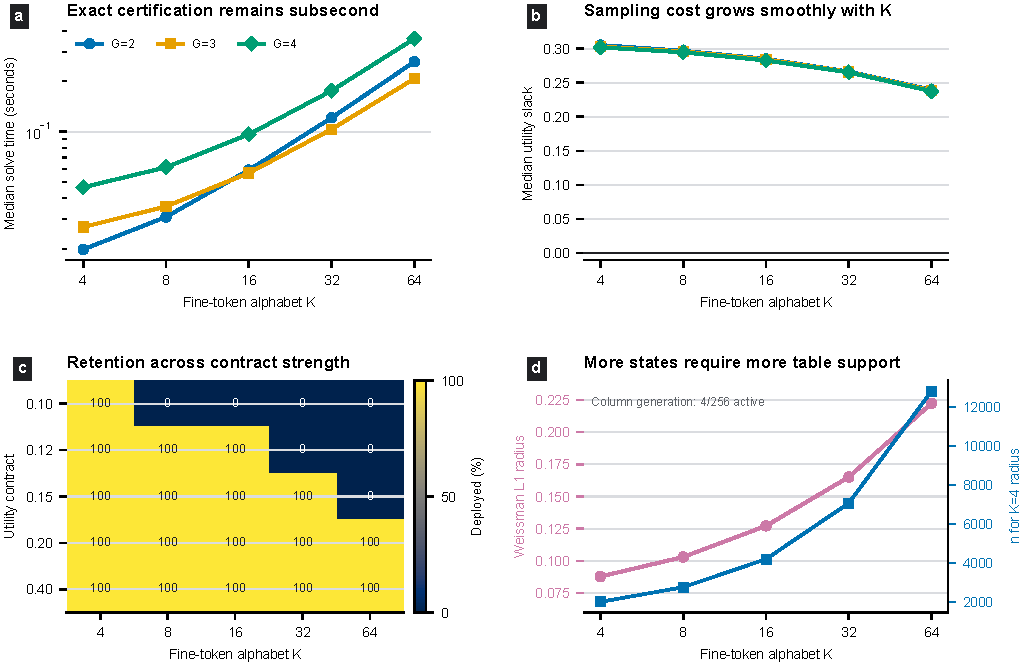
\includegraphics[width=\textwidth]{figures/figure5_mosaic_scaling.pdf}
  \caption{Finite-alphabet scaling over five independent tables per cell.
  (a) Median wall-clock optimization. (b) Median utility slack at the $.40$
  contract. (c) Retention averaged over $G=2,3,4$ at tighter contracts.
  (d) The Weissman radius and per-stratum sample size needed to recover the
  $K=4$ radius for $G=4$. A $G=L=4$ constraint-generation stress uses 4 of
  256 possible attacker assignments.}
  \label{supp:fig:scaling}
\end{figure*}

\begin{table*}[t]
\centering
\small
\setlength{\tabcolsep}{4.0pt}
\begin{tabular}{rrrrrr}
\hline
$K$ & Median time (s) & $\ell_1$ radius & Utility slack & Retained at $.40$ & $n$ for $K=4$ radius \\
\hline
4  & .047 & .0878 & .3019 & 5/5 & 2,000 \\
8  & .062 & .1030 & .2945 & 5/5 & 2,752 \\
16 & .097 & .1271 & .2826 & 5/5 & 4,192 \\
32 & .174 & .1651 & .2652 & 5/5 & 7,067 \\
64 & .360 & .2223 & .2374 & 5/5 & 12,817 \\
\hline
\end{tabular}
\caption{$G=4$ scaling summary; the complete artifact also contains $G=2,3$.
The synthetic tables isolate computation and confidence-radius scaling.}
\label{supp:tab:scaling}
\end{table*}
